\HeaderQuote{Well! I've often seen a cat without a grin; but a grin without a 
cat! It's the most curious thing I ever say in my life!}{Alice} 

\chapter{Generating Training Data}\label{ch:gentrdat} 

\FirstSentence{W}{hen building a complete} \jsp\ schedule, $K=n\cdot m$ 
dispatches must be made sequentially.
A job is placed at the earliest available time slot for its next machine, 
whilst still fulfilling constraints \cref{eq:permutation,eq:oneJobPerMac}.
%that each machine can handle at most one job at each time, and jobs need to 
%have finished their previous machines according to its machine order. 
Unfinished jobs are dispatched one at a time according to some heuristic, or 
policy $\pi$. 
After each dispatch\footnote{The terms dispatch (iteration) and time step are 
    used interchangeably.} the schedule's current features (cf. 
\cref{tbl:features}) are updated based on the half-finished schedule. Namely, 
when implementing \cref{pseudo:constructJSP}, a training set will consist of 
all features from \cref{tbl:features} at every post-decision state visited in 
line \ref{pseudo:constructJSP:phi}. 
These collected features are denoted $\Phi$, where, 
\begin{equation}\label{eq:Phi}
\Phi:= \bigcup_{i=1}^{N_{\text{train}}} 
\bigcup_{k=1}^K\bigcup_{J_j\in\mathcal{L}^{(k)}} 
\condset{\vphi_j}{\vec{x}_i\in\mathcal{P}^{n\times m}_{\text{train}} }.
\end{equation}

\begin{figure}[p]
      \begin{tikzpicture}
  \node[anchor=south west,inner sep=0] (image) at (0,0,0) 
  {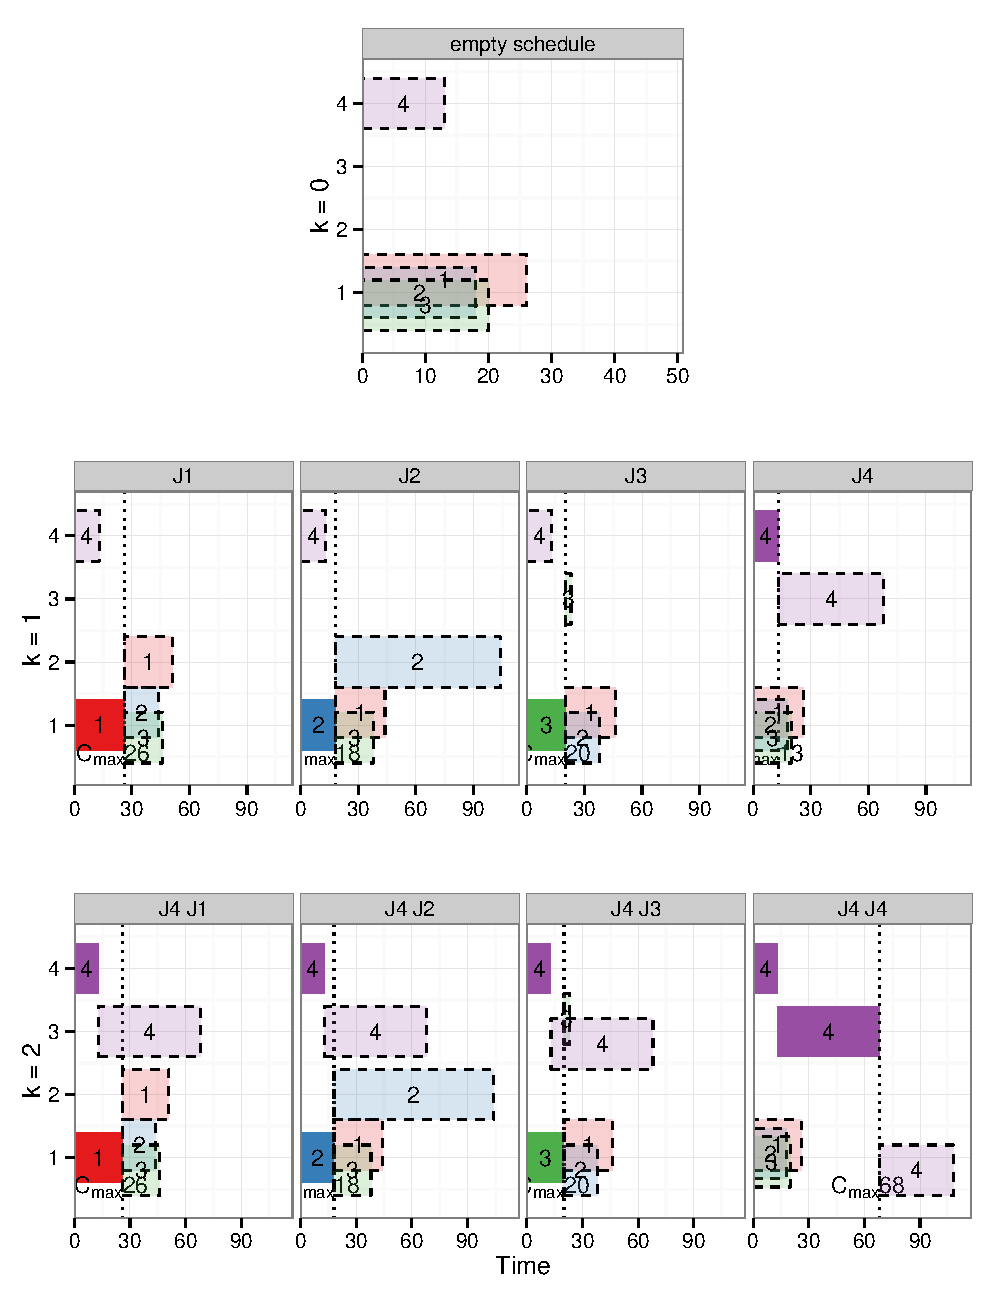
\includegraphics[width=\textwidth]{gametree}};
  \begin{scope}[x={(image.south east)},y={(image.north west)}]
  %% next four lines will help you to locate the point needed by forming a 
  %%grid. comment these four lines in the final picture.↓
  %\draw[help lines,xstep=.1,ystep=.1] (0,0) grid (1,1);
  %\draw[help lines,xstep=.05,ystep=.05] (0,0) grid (1,1);
  %\foreach \x in {0,1,...,9} { \node [anchor=north] at (\x/10,0) {0.\x}; }
  %\foreach \y in {0,1,...,9} { \node [anchor=east] at (0,\y/10) {0.\y};}
  %% upto here↑
  \node (J0) at (0.5,0.71) {};
  \node (J1) at (0.19,0.65) {};
  \node (J2) at (0.42,0.65) {};
  \node (J3) at (0.65,0.65) {};
  \node (J4) at (0.85,0.65) {};
  \draw[-latex] (J0) to[out=-20,in=+20] (J1);
  \draw[-latex] (J0) to[out=-20,in=+20] (J2);
  \draw[-latex] (J0) to[out=-20,in=+20] (J3);
  \draw[-latex] (J0) to[out=-20,in=+20] (J4);
  \node (J4) at (0.82,0.38) {};
  \node (J4J1) at (0.19,0.31) {};
  \node (J4J2) at (0.42,0.31) {};
  \node (J4J3) at (0.65,0.31) {};
  \node (J4J4) at (0.85,0.31) {};
  \draw[-latex] (J4) to[out=-20,in=+20] (J4J1);
  \draw[-latex] (J4) to[out=-20,in=+20] (J4J2);
  \draw[-latex] (J4) to[out=-20,in=+20] (J4J3);
  \draw[-latex] (J4) to[out=-20,in=+20] (J4J4);
  \end{scope}
  \end{tikzpicture}

    \vspace{-27pt}
    \caption[Partial Game Tree for \jsp]{Partial Game Tree for \jsp\ for the 
        first two dispatches. 
        Top layer depicts all possible dispatches (dashed) for an empty 
        schedule. 
        Middle layer depicts all possible dispatches given that one of the 
        dispatches from the layer above has been executed (solid). 
        Bottom layer depicts when job $J_4$ on machine $M_4$ has been chosen to 
        be dispatched from the previous layer, moreover it depicts all possible 
        next dispatches from that scenario.}
    \label{fig:example:gametree}
\end{figure}

\vspace*{-24pt}
\section{\Jsp\ tree representation}\label{sec:gen:gametree}
Continuing with the example from \cref{sec:jsp:example}, 
\cref{fig:example:gametree} shows how the first two dispatches could be 
executed for a $4\times5$ \jsp\ from \cref{sec:jsp:example}.
In the top layer one can see an empty schedule.
In the middle layer one of the possible dispatches from the layer above is 
fixed, and one can see the resulting schedule, i.e., what are the next possible 
dispatches given this scenario? Assuming $J_4$ would be dispatched first, the 
bottom layer depicts all the next possible partial schedules.

This sort of tree representation is similar to \emph{game trees} 
\citep[cf.][]{Rosen03} where the root node denotes the initial (i.e. empty) 
schedule and the leaf nodes denote the complete schedule (resulting after 
$n\cdot m$ dispatches, thus height of the tree is $K$), therefore the 
distance $k$ from an internal node to the root yields the number of operations 
already dispatched. Traversing from root to leaf node one can obtain a sequence 
of dispatches that yielded the resulting schedule, i.e., the sequence indicates 
in which order the tasks should be dispatched for that particular schedule. 

\section{Labelling schedules w.r.t. optimal decisions} 
%\label{sec:trdat:label}
One can easily see that sequence $\vchi$ from \cref{eq:vchi} for task 
assignments is by no means unique. 
Inspecting a partial schedule further along in the dispatching process such as 
in \cref{fig:example:midway}, then let's say $J_2$ would be dispatched next, 
and in the next iteration $J_4$. 
Now this sequence would yield the same schedule as if $J_4$ would have been 
dispatched first and then $J_2$ in the next iteration. 
This is due to the fact they have non-conflicting machines, which indicates 
that some of the nodes in game tree can merge. 
Meanwhile, the states of the schedule are different and thus their 
features, although they manage to yield with the same (partial) schedule at a 
later date.  % ATHUGASEMD 1 -- SEQ. REP NON-UNIQUE
In this particular instance one can not infer that choosing $J_2$ is better and 
$J_4$ is worse (or vice versa) since they can both yield the same solution.

Furthermore, in some cases there can be multiple optimal solutions to the same 
problem instance. 
Hence not only is the sequence representation `flawed' in the sense that slight 
permutations on the sequence are in fact equivalent w.r.t. the end-result.
In addition, varying permutations of the dispatching sequence (however given 
the same partial initial sequence) can result in very different complete 
schedules but can still achieve the same makespan, and thus same \fullnamerho\ 
(which is the measure under consideration). 
Care must be taken in this case that neither resulting features are labelled as 
undesirable. 
Only the features from a dispatch yielding a truly suboptimal solution should 
be labelled undesirable. 

\section{Computational growth}
The creation of the game tree for \JSP\ can be done recursively for all 
possible permutations of dispatches, resulting in a full \mbox{$n$-ary} tree 
(since $|\mathcal{L}|\leq n$) of height $K$. 
Such an exhaustive search would yield at the most $n^K$ leaf nodes (worst case 
scenario being no sub-trees merge). Since the internal vertices (i.e. 
partial schedules) are only of interest to learn,\footnote{The root is 
  the empty initial schedule and for the last dispatch there is only one option 
  left to choose from, so there is no preferred `choice' to learn.} 
the number of those can be at the most \mbox{${}^{n^K-1}/_{n-1}$}.
Even for small dimensions of $n$ and $m$ the number of internal vertices are 
quite substantial and thus too computationally expensive to investigate them 
all. Not to mention that this is done iteratively for all $N_{\text{train}}$ 
problem instances.

Since we know that once a job is processed on all of its machines, then it 
stops being a contender for future dispatches, therefore the all possible 
assignments of operations for an $n\times m$~~\JSP\ would require an 
examination of $(n!)^m$ \citep{Giffler60}, thus a $6\times5$ problem may have 
at most $1.93\cdot10^{14}$ possible solutions, and for $10\times10$ problem 
then it's $3.96\cdot10^{65}$ solutions! Thus the factorial growth makes it 
infeasible for exploring all nodes to completion. However, our training data 
consist of relatively large $N_{\text{train}}$, so even though we will only 
pursue one trajectory per instance, then the aggregated training data will give 
it variety.

\section{Trajectory sampling strategies}\label{sec:trdat:tracks}
For each feature in \cref{eq:Phi} we need to keep track of the resulting 
makespan for its dispatched job. 
As a result, we obtain the meta-data $\{\Phi,\mathcal{Y}\}$ from 
\cref{fig:rice} as follows, 
\begin{equation}\label{eq:trdat:metadata}
\condset{\{ \vphi_j, C_{\max}^{\pi_\star(\vchi^j)}
    \}}{J_j\in\mathcal{L}^{(k)}}_{k=1}^K \in \Phi \times \mathcal{Y}
\end{equation}
for a single problem instance $\vec{x}\in\mathcal{P}_{\text{train}}$, and where 
$C_{\max}^{\pi_\star(\vchi^j)}$ denotes the optimal makespan (i.e. following 
the expert policy $\pi_\star$) from the resulting post-decision state $\vchi^j$.

Due to superabundant possible solutions for a single problem instance, 
there needs to be some logic based on how to sample the state-space for a 
valuable outcome. Especially considering the cost of correctly labelling 
\footnote{Optimal solutions can be obtained by using a commercial software 
    package by \citet{gurobi}, which has a free academic licence. However, GLPK 
    by \citet{glpk} has a free licence. Alas, GLPK has a lacklustre performance 
    w.r.t. speed for solving $10\times10$ \JSP.}
each dispatch that is encountered.\footnote{Generally it takes 
    only several hours to collect $N_{\text{train}}^{6\times5}=500$. Alas, when 
    going to higher dimension, $N_{\text{train}}^{10\times10}=300$ 
    really becomes an issue, as \jrnd{10}{10} needs a few days, and 
    \jrndn{10}{10} or \frnd{10}{10} require several weeks!}
Obviously we'd like to inspect optimal solutions as they are what we'd like to 
mimic. Moreover, since we'd like to infer the footprints in instance space for 
the SDRs we started doing in \cref{ch:defdifficulty}, then we will consider 
them also.
Similarly, the weights for \cref{eq:CDR:feat} that were optimised directly 
using from evolutionary search (cf. \cref{ch:esmodels}) will also be used.

\clearpage
To clarify, the trajectory sampling strategies for collecting a feature set and 
its corresponding labelling for \cref{eq:trdat:metadata} are the following:
\begin{description}
    \item[Optimum trajectory, \PhiSet{OPT},] at each dispatch some (random) 
    optimal task is dispatched. This is also referred to following the expert 
    policy, $\pi_\star$.
    \item[SPT trajectory, \PhiSet{SPT},] at each dispatch the task 
    corresponding to shortest processing time is dispatched, i.e., following 
    \sdr~SPT.
    \item[LPT trajectory, \PhiSet{LPT},] at each dispatch the task 
    corresponding to largest processing time is dispatched, i.e., following 
    \sdr~LPT.
    \item[LWR trajectory, \PhiSet{LWR},] at each dispatch the task 
    corresponding to least work remaining is dispatched, i.e., following 
    \sdr~LWR.
    \item[MWR trajectory, \PhiSet{MWR},] at each dispatch the task 
    corresponding to most work remaining is dispatched, i.e., following 
    \sdr~MWR.
    \item[Random trajectory, \PhiSet{RND},] at each dispatch some random task 
    is dispatched.
    \item[CMA-ES trajectory, $\Phi^{\minRho}$,] at each dispatch the task 
    corresponding to highest priority, computed with fixed weights $\vec{w}$, 
    which were obtained by optimising the mean for \fullnamerho, with CMA-ES 
    optimisation from \cref{ch:esmodels}. 
    \item[All trajectories, \PhiSet{ALL},] denotes all aforementioned 
    trajectories were explored, i.e., \vspace*{-18pt}
    \begin{equation}
    \Phi^{\text{ALL}}:=\condset{\Phi^{A}}{\forall A \in 
    \left\{\text{OPT,~SPT,~LPT,~LWR,~MWR,~RND,~}\minRho\right\}}
    \end{equation}
\end{description}

When following optimal trajectory, then due to the nature of the sequence 
representation (i.e. $\vchi$), the earlier stages for \Problem{j.rnd} of the 
dispatching are more or less equivalent and thus irrelevant (cf. 
\cref{fig:diff:case:OPT}). 
Hence it is appropriate to follow some random optimal path to begin with and 
then go after some (if not all possible) optimal paths until completion at step 
$K$. 

In the case of the $\Phi^{\langle \text{SDR} \rangle}$ and $\Phi^{\minRho}$ 
trajectories it is sufficient to explore each trajectory exactly once for each 
problem instance. 
Whereas, for \PhiSet{OPT} and \PhiSet{RND} there can be several 
trajectories worth exploring, however, only one is chosen (at random). It is 
noted that since the number of problem instances, $N_{\text{train}}$, is 
relatively large, it is deemed sufficient to explore one trajectory for each 
instance, in those cases as well.

These trajectory strategies were initially introduced in \cref{InRu15a}. 
However, more SDR-based trajectories are now addressed since, e.g., LWR is 
considered more favourable for \fsp\ rather than MWR (cf. 
\cref{ch:defdifficulty}). 

The number of features that were collected on a step-by-step basis for 
\Problem[6\times5]{\text{train}} in \cref{tbl:data} is illustrated in 
\cref{fig:size:trdat}. 
There is an apparent stair-like structure for LWR, in accordance with its 
motivation (cf. \cref{sec:SDR}), which is completing jobs advanced in their 
progress, that is to say minimising $\mathcal{L}$ and from \cref{eq:Phi} we 
have $\abs{\Phi}\propto\abs{\mathcal{L}}$.
Whereas MWR tries to keep the jobs more balanced, hence more steady 
$\abs{\mathcal{L}}$, until at $k>(K-n)$ then \mbox{$\abs{\mathcal{L}} \lneq 
(K-k)$}, which explains the sharp decent near the end for MWR.
\Cref{tbl:size:trdat} gives the total size for $\abs{\Phi}$, indicating the
number of optimisations needed for obtaining $\mathcal{Y}$.

\begin{figure}[t]
    \includegraphics[width=\textwidth]{{trdat.size.6x5}.pdf}
    \vspace{-24pt}
    \caption[Size of training set, $\abs{\Phi}$]{Size of training set, 
        $\abs{\Phi}$, for different trajectory strategies 
        ($N_{\text{train}}=500$)}
    \label{fig:size:trdat}
\end{figure}

\begin{table}[b]\centering
    \caption{Total number of features in $\Phi$ for all $K$ steps}
    \label{tbl:size:trdat}
    \vspace{-12pt}
{\setlength{\tabcolsep}{2pt} \scriptsize
\subcaptionbox{\Problem[6\times5]{\text{train}}, $N_{\text{train}}=500$}{
\begin{tabular}{lccccccccc}
  \toprule
  Track & 
  $j.rnd$ & $j.rndn$ & $j.rnd,J_1$& $j.rnd,M_1$ & $f.rnd$ & $f.rndn$ & $f.jc$ & 
  $f.mc$ & $f.mxc$ \\ 
  \midrule
  SPT & 63197 & 63074 & 64560 & 61320 & 63287 & 63123 & 53678 & 66995 & 66216 \\
  LPT & 63516 & 63374 & 63595 & 62864 & 63535 & 63320 & 53746 & 66356 & 65662 \\
  LWR & 52500 & 52500 & 52500 & 52500 & 52500 & 52500 & 52500 & 52500 & 52500 \\
  MWR & 79230 & 82500 & 78327 & 77934 & 79288 & 82500 & 80546 & 82498 & 82485 \\
  RND & 71390 & 71608 & 71445 & 71463 & 71427 & 71945 & 71558 & 71456 & 71649 \\
  OPT & 76592 & 78176 & 74109 & 74069 & 70037 & 69180 & 69716 & 71602 & 71102 \\
  $\minRho$ & 79319 & 81423 & 79070 & 78501 & 72866 & 56428 & 60049 & 52710 & 
  57177 \\
  \bottomrule
\end{tabular}}
\subcaptionbox{\Problem[10\times10]{\text{train}}, $N_{\text{train}}=300$}{
\begin{tabular}{lccc}
  \toprule
  Track & $j.rnd$ & $j.rndn$ & $f.rnd$ \\ 
  \midrule
  SPT & 211351 &     -- &     -- \\ 
  LPT & 210490 &     -- &     -- \\ 
  LWR & 165000 &     -- &     -- \\ 
  MWR & 280739 &     -- &     -- \\ 
  RND & 252515 &     -- &     -- \\ 
  OPT & 272858 & 245313 & 211763 \\ 
  \bottomrule
\end{tabular}
}}
\end{table}
